% This file is part of the multi-tex ECE 486 Final Project Report 
% file name: 3-full-state-feedback-control-friction-compensation.tex

% YOU DO NOT COMPILE FROM THIS SINGLE FILE, read the following

% included files:
% (Makefile)
% Makefile -- run make Makefile (on Mac or Linux), it takes care of LaTeX compilation

% (*.PDF)
% report.pdf -- report file, print it out and submit it

% (*.TEX)
% report.tex -- main file, pdflatex this file (tested on Mac and Linux)
% 0-title-page.tex -- title page 
% 1-introduction.tex -- chapter 1 
% 2-mathematical-model.tex -- chapter 1 (lagrange equations of motion) and chapter 4 (linearisation)
% 3-full-state-feedback-control-friction-compensation.tex -- (this file) chapter 2 and chapter 4 (two state and three state feedback controller design) 
% 4-full-state-feedback-control-decoupled-observer.tex -- chapter 4 (controller design) and chapter 5 (observer design for estimated state)
% 5-conclusions.tex -- conclusion
% 6-extra-credit.tex -- (optional) add thsese pages if you have demoed chapter 6 and chapter 7

\section{Full State Feedback Control with Friction Compensation}
Using the models we derived from above, we were then able to design the compensators to stabilize our system.
\subsection{Development of the PD Control with Friction Compensation}
We want to stabilize this system with a PD controller. Since this is a relatively big matrix we wanted to introduce some simplifications to it. We first reduced our system to a second order system using only the position for the pendulum and its derivative. This results in the following model:

$$
\begin{bmatrix}
\delta\dot\theta_p\\
\ddot\theta_p
\end{bmatrix}
=
\begin{bmatrix}
0 & 1\\
a & 0
\end{bmatrix}
\begin{bmatrix}
\delta\theta_p\\
\dot\theta_p
\end{bmatrix}
+
\begin{bmatrix}
0\\
-b_p
\end{bmatrix}
u$$

We then had to pick our desired poles for the closed loop system. We were given the requirements of having an $\omega_n > \omega_{np}$ and a $\zeta < \frac{1}{\sqrt{2}}$. We picked the following values: $\omega_n = 10$ and $\zeta = 0.5$. This resulted in these poles: $(3^\frac{1}{2}*5*j - 5)$,$(-3^\frac{1}{2}*5*i - 5)$.

From this we can use the MATLAB ``place'' function to generate the desired control matrix.

We also tried increasing the complexity and introduced the rotor speed into our control as well. In our three state feedback, we added an extra pole at -5, in between our previous poles and one at 0.

Like our two state control, our three state model is as follows:

$$
\begin{bmatrix}
\delta\dot\theta_p\\
\ddot\theta_p\\
\delta\dot\theta_r\\
\ddot\theta_r
\end{bmatrix}
=
\begin{bmatrix}
0 & 1 & 0 & 0\\
a & 0 & 0 & 0\\
0 & 0 & 0 & 1\\
0 & 0 & 0 & 0
\end{bmatrix}
\begin{bmatrix}
\delta\theta_p\\
\dot\theta_p\\
\delta\theta_r\\
\dot\theta_r
\end{bmatrix}
+
\begin{bmatrix}
0\\
-b_p\\
0\\
b_r
\end{bmatrix}
u$$

Our poles were $(3^\frac{1}{2}*5*j - 5)$,$(-3^\frac{1}{2}*5*i - 5)$,$5$,$0$.

Finally, we included friction compensation. In order to do this, we needed to experimentally find our firction coeeficients. We know that friction can be modeled as viscous and coulob friction in the form of $b\dot\theta_r+c$. Since this is a linear relationship, we were able to test our rotor at multiple speeds and calculate these coefficients from linear fits of our resulting data. Experiementaly however, we discovered that friction compensation was not benificial because the friction allowed us to have damping effects and kept the pendulum from swaying as much.

\begin{figure}
  \caption{Our control block diagram of our three-state feedback with friction compensation}
  \centering
    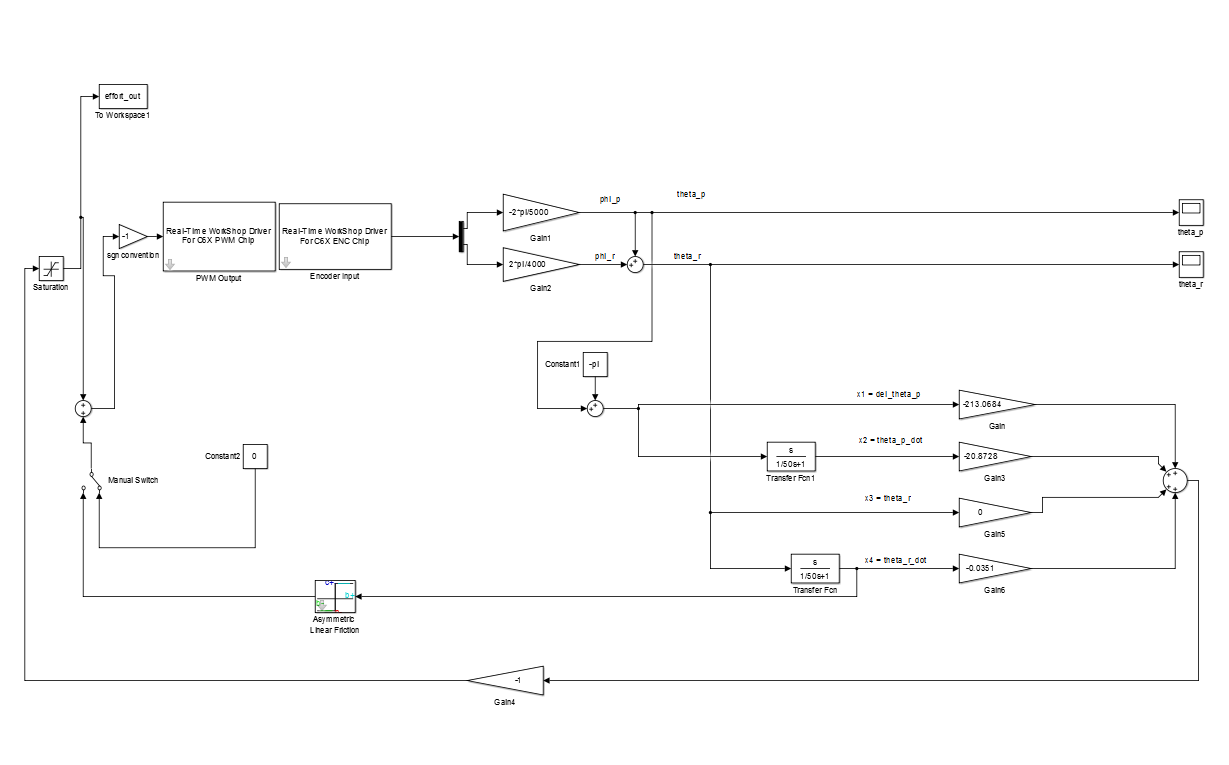
\includegraphics[scale = 0.4]{three_state.PNG}
\end{figure}

\subsection{Mathematical Proof}
We want to prove though that this does indeed create a stable system.

Our system can be described as follows:
$\boldsymbol{\dot x = Ax+B}u$

$$
\begin{bmatrix}
\delta\dot\theta_p\\
\ddot\theta_p\\
\delta\dot\theta_r\\
\ddot\theta_r
\end{bmatrix}
=
\begin{bmatrix}
0 & 1 & 0 & 0\\
a & 0 & 0 & 0\\
0 & 0 & 0 & 1\\
0 & 0 & 0 & 0
\end{bmatrix}
\begin{bmatrix}
\delta\theta_p\\
\dot\theta_p\\
\delta\theta_r\\
\dot\theta_r
\end{bmatrix}
+
\begin{bmatrix}
0\\
-b_p\\
0\\
b_r
\end{bmatrix}
u$$

We designed the pole locations of the closed-loop system to be at $(3^\frac{1}{2}*5*j - 5)$,$(-3^\frac{1}{2}*5*i - 5)$,$5$,$0$ in order to satisfy the transient response requirements. All the poles are in the LHP and hence stable. Using place command, we get the controller to be [-213 -20.8 0 -0.0351].Rewriting the system equation to be:
$\boldsymbol{\dot x = Ax+B}u$

$$
\begin{bmatrix}
\delta\dot\theta_p\\
\ddot\theta_p\\
\delta\dot\theta_r\\
\ddot\theta_r
\end{bmatrix}
=
\begin{bmatrix}
0 & 1 & 0 & 0\\
-150 & -21.8 & 0 & -0.0367\\
0 & 0 & 0 & 1\\
41597 & 4075 & 0 & 6.8476
\end{bmatrix}
\begin{bmatrix}
\delta\theta_p\\
\dot\theta_p\\
\delta\theta_r\\
\dot\theta_r
\end{bmatrix}
$$

At steady state, the $\dot x$ should be zero. Setting $\dot x$ to 0 and using Matlab, we computed the solution of the equation to be $[0 0 0 0]^T$. This means that  $\delta\theta_p=0$ $\dot\theta_p=0$  $\dot\theta_r=0$  are the only stable equilibrium for the equation.  This means that the system will stablize to the inverted position at steady state.

\subsection{Robustness Comparisons}
The following table shows our simulated robustness results. One can see that our three state feedback was able to withstand the largest pulse and disturbance forces and still stay stable.\\
\begin{tabular}{|c|c|c|c|}
\hline
 & Two-state Feedback & Three-state Feedback & Observer\\ \hline
 & $\delta\theta_p$  $\delta\theta_r$ & $\delta\theta_p$  $\delta\theta_r$ & $\delta\theta_p$  $\delta\theta_r$\\ \hline
Max IC deviations & 0.12  1.1 & 0.12  1 & 0.12  0.99\\ \hline
Max pulse & 7.5 & 8.1 & 7\\ \hline
Max disturbance & 5 & 7.4 & 6.3\\
\hline
\end{tabular}
\subsection{System Behavior}
With the controller, the system will be stabilized at the equilibrium point $\theta_p= \pi$. From the Windows Target implementation, we see that the system is able to adjust and stabilize to the top position with small initial deviations. It could also reject gentle tap which represent a pulse disturbance as well as the constant disturbance. As such, the system is stabilized by the controller we designed at the top position and it has certain degree of robustness to resist disturbances. We also took note that frictional forces here benefit us and damps out distrubances.